\scanpage{71}
\mspage{\deleted{\unsure{69|79}}\unsure{70|79}}

Il revient au $=$ de dire que $F$ et $F'$ ont $=$ cosupport, ou encore, même support.

\unsure{Donnons nous} un support.

% fig:margin-mark-columns. Literal separated ink fragments; their function is uncertain.
\margin{\figure{\begin{tikzpicture}[x=0.7cm,y=0.7cm]
\fill (0.03,0.32) ellipse (0.025 and 0.035);
\draw[line width=0.75pt] (0.02,0.26) -- (0.02,0.13) -- (0.045,0.10);
\fill (0.01,0.05) ellipse (0.025 and 0.025);
\draw[line width=0.75pt] (0.035,0.015) .. controls (0.07,-0.06) and (0.00,-0.12) .. (0.025,-0.19);
\fill (0.12,-0.28) circle (0.028);
\fill (1.94,0.65) ellipse (0.021 and 0.029);
\draw[line width=0.7pt] (1.96,0.58) -- (1.97,0.52) -- (1.93,0.49);
\fill (1.97,0.41) circle (0.024);
\fill (1.97,0.31) circle (0.023);
\fill (1.94,0.12) circle (0.027);
\end{tikzpicture}}}
Une autre façon de dire que $F,G\ \text{disj.}\Longrightarrow F',G\ \text{disj}$, est ainsi :

% The one rising stroke cancels de beneath the raised phrase.
\uline{Corollaire} Le cosupport \deleted{de} \inserted{dans $\unsure{F|\mathcal F}$} tout objet $G$ de $\mathcal F$ est fermé, non \unsure{seult|seulemt} pour $\leq$, mais aussi pour $\preceq$ -- c'est donc ce qu'on appelle une \uline{sous}-\unsure{contrée|contrie}.

Donc \unsure{itou} pour toute partie $\Phi\subset\mathcal F$.

En d'autres termes, \deleted{toute} partie de $\mathcal F$ qui est un $\mathcal F$-support (ou ``$\mathcal F$-\unsure{saturee|saturée}, sous-entendu : en termes de $\leq$\unsure{,)|,)\}|,) ;} cf \unsure{page|pge} $67$) est \unsure{automatiquemt|automatiquement} \deleted{\unsure{f}}une sous-contrée.

% The following number and cancelled draft are upside down on the sheet.
\mspage{\deleted{5\deleted{\unsure{4|3}}5}}

% fig:inverted-cancelled-draft. Text occurs once, in the same group as the boundary and oblique cancellation strokes.
% The isolated glyph under the first Phi is not securely separable from its retracing.
\figure{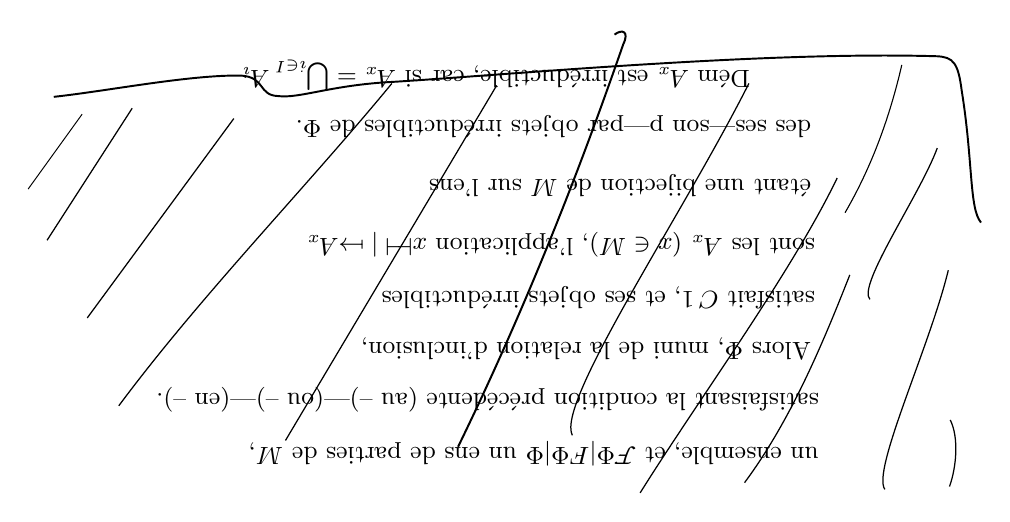
\begin{tikzpicture}[x=0.005cm,y=-0.005cm,font=\small]
\begin{scope}[rotate=180,transform shape]
\node[anchor=base west,inner sep=0pt] at (410,220) {\deleted{un ensemble, et $\unsure{\deleted{\mathcal F}\Phi|\deleted{F}\Phi|\Phi}$ un ens de parties de $M$,}};
\node[anchor=base west,inner sep=0pt] at (410,355) {\deleted{satisfaisant la condition précédente \unsure{(au --)|(ou --)|(en --)}.}};
\node[anchor=base west,inner sep=0pt] at (430,485) {\deleted{Alors $\Phi$, muni de la relation d'inclusion\unsure{,}}};
\node[anchor=base west,inner sep=0pt] at (420,615) {\deleted{satisfait $C\,1$, et ses objets irréductibles}};
\node[anchor=base west,inner sep=0pt] at (420,750) {\deleted{sont les $A_x$ $(x\in M)$, l'application $x\unsure{\mathrel{\vdash\joinrel\dashv}|\mapsto} A_x$}};
\node[anchor=base west,inner sep=0pt] at (430,900) {\deleted{étant une bijection de $M$ sur l'ens}};
\node[anchor=base west,inner sep=0pt] at (430,1050) {\deleted{des \deleted{\unsure{ses|son} \unsure{p|par}} objets irréductibles de $\Phi$.}};
\node[anchor=base west,inner sep=0pt] at (585,1177) {\deleted{\unsure{Dém} $A_x$ est irréductible, car si $A_x=\bigcup_{i\in I} A_i$}};
% The boundary is open at the scan edge; its upper continuation is not inferred.
\draw[line width=0.7pt] (0,790) .. controls (30,825) and (20,945) .. (49,1125)
 .. controls (58,1195) and (70,1210) .. (112,1212)
 .. controls (550,1225) and (1200,1165) .. (1492,1147)
 .. controls (1650,1139) and (1730,1104) .. (1784,1111)
 .. controls (1835,1113) and (1815,1159) .. (1878,1163)
 .. controls (2010,1165) and (2215,1124) .. (2353,1109);
% Thirteen distinct oblique or curved cancellation strokes.
\draw[line width=0.45pt] (80,120) .. controls (62,170) and (56,245) .. (78,289);
\draw[line width=0.45pt] (244,113) .. controls (278,160) and (130,475) .. (83,669);
\draw[line width=0.45pt] (282,595) .. controls (315,630) and (155,860) .. (111,979);
\draw[line width=0.45pt] (600,130) .. controls (485,285) and (405,474) .. (333,657);
\draw[line width=0.45pt] (865,104) .. controls (720,336) and (480,664) .. (365,903);
\draw[line width=0.40pt] (345,815) .. controls (276,934) and (231,1060) .. (201,1190);
\draw[line width=0.45pt] (1037,250) .. controls (1080,332) and (758,808) .. (589,1143);
\draw[line width=0.72pt] (1327,221) .. controls (1130,625) and (993,997) .. (908,1242)
 .. controls (892,1275) and (910,1282) .. (930,1267);
\draw[line width=0.45pt] (1765,237) -- (1229,1138);
\draw[line width=0.45pt] (2188,325) .. controls (1978,607) and (1714,877) .. (1495,1143);
\draw[line width=0.45pt] (2268,548) -- (1896,1054);
\draw[line width=0.45pt] (2370,745) -- (2154,1080);
\draw[line width=0.35pt] (2418,875) -- (2281,1065);
\end{scope}
\end{tikzpicture}}
